Once the tree is available, we automatically optimize the schedule for traversing a tree level in a way that avoids instruction divergence. Our insight is that we can cluster tasks (nodes) based on node attributes that influence control flow. We match the data layout to the new schedule, and optimize the clustering process to prevent the planning overhead to outweigh its benefit. The overall optimization can be thought of an extension to loop unswitching where the predicate is input-dependent and a sorting prepass guarantees that subintervals will branch identically.

\begin{figure}
\subfloat{  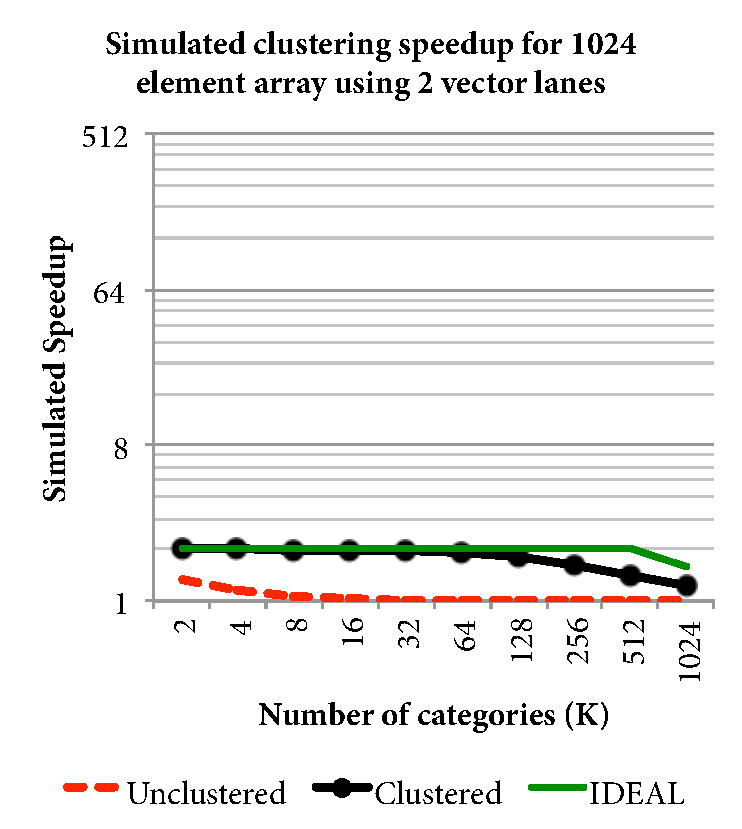
\includegraphics[trim=0 0 0 0,clip,width=0.32\columnwidth]{chapter6/simulatedclusteringspeedup/simulatedclusteringspeedup-1} }
\subfloat{  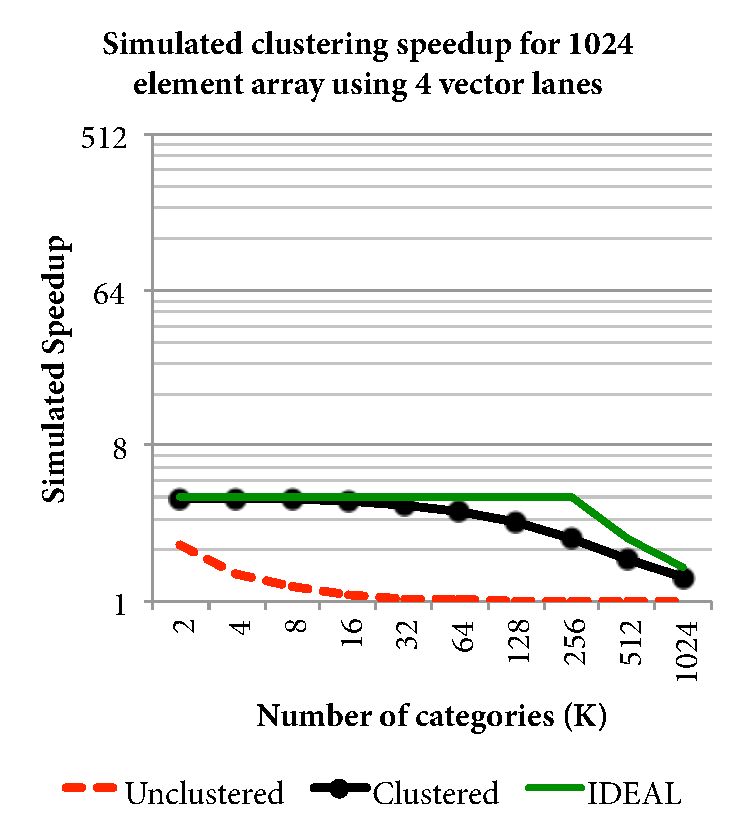
\includegraphics[trim=0 0 0 0,clip,width=0.32\columnwidth]{chapter6/simulatedclusteringspeedup/simulatedclusteringspeedup-2} }
\subfloat{  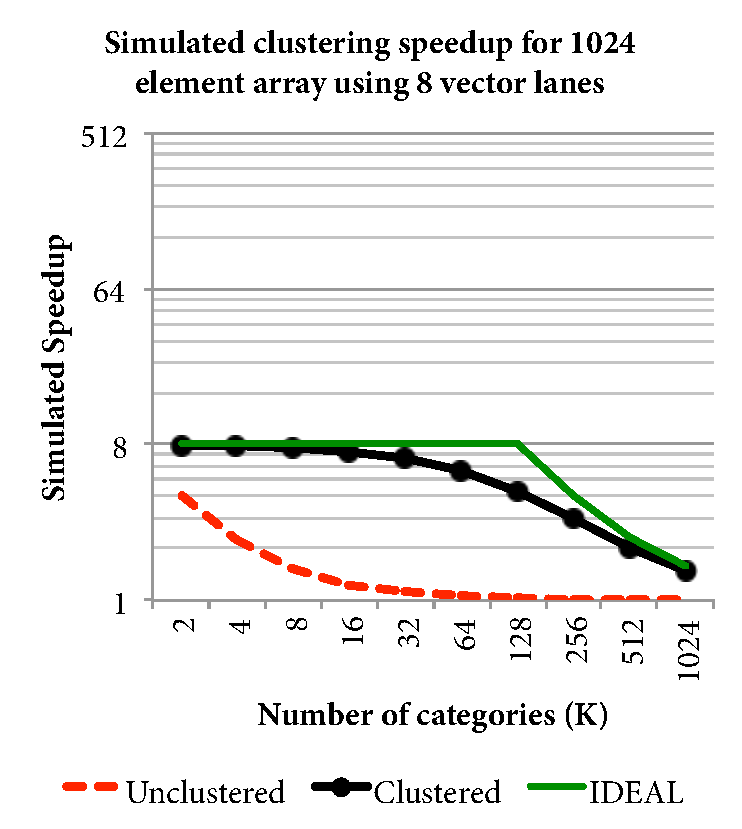
\includegraphics[trim=0 0 0 0,clip,width=0.32\columnwidth]{chapter6/simulatedclusteringspeedup/simulatedclusteringspeedup-3} } \\
\subfloat{  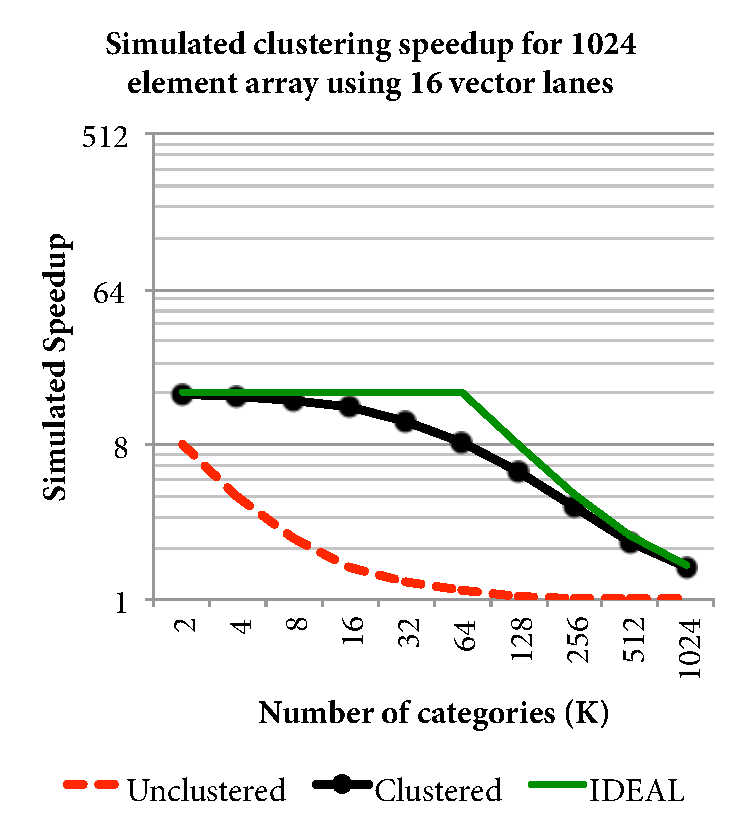
\includegraphics[trim=0 0 0 0,clip,width=0.32\columnwidth]{chapter6/simulatedclusteringspeedup/simulatedclusteringspeedup-4} }
\subfloat{  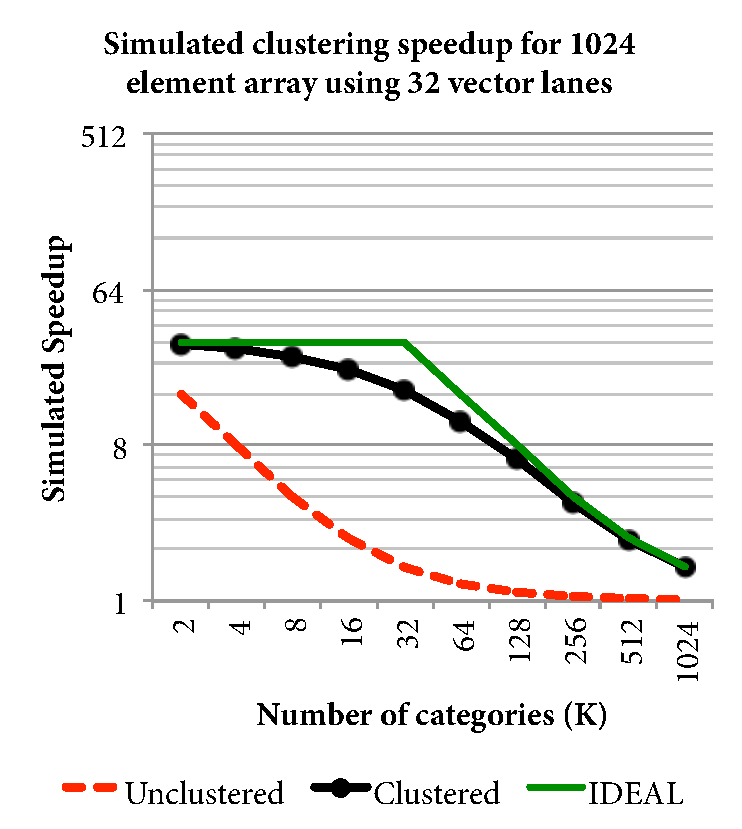
\includegraphics[trim=0 0 0 0,clip,width=0.32\columnwidth]{chapter6/simulatedclusteringspeedup/simulatedclusteringspeedup-5} }
\subfloat{  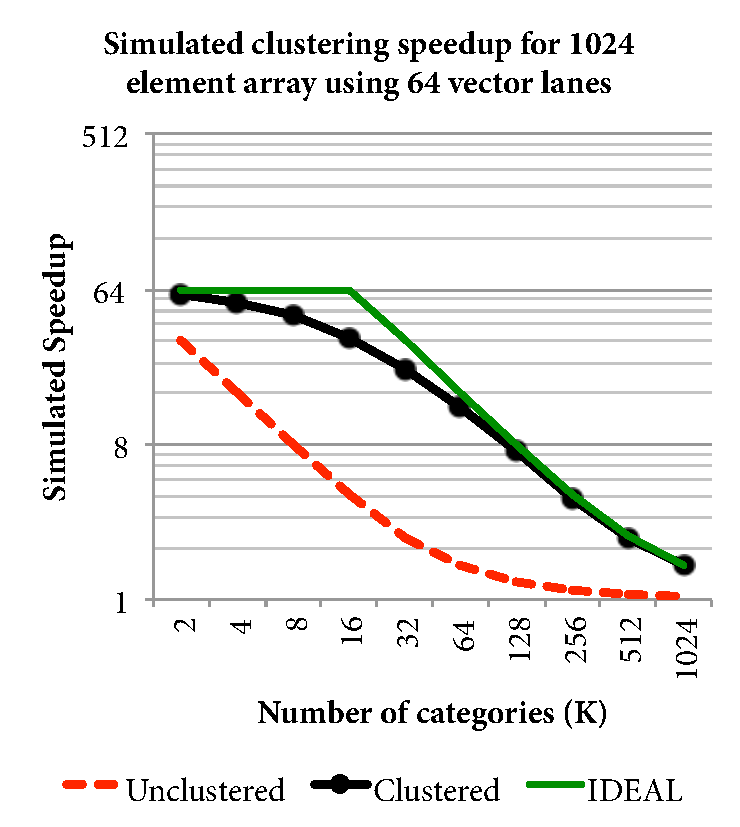
\includegraphics[trim=0 0 0 0,clip,width=0.32\columnwidth]{chapter6/simulatedclusteringspeedup/simulatedclusteringspeedup-6} } \\
\subfloat{  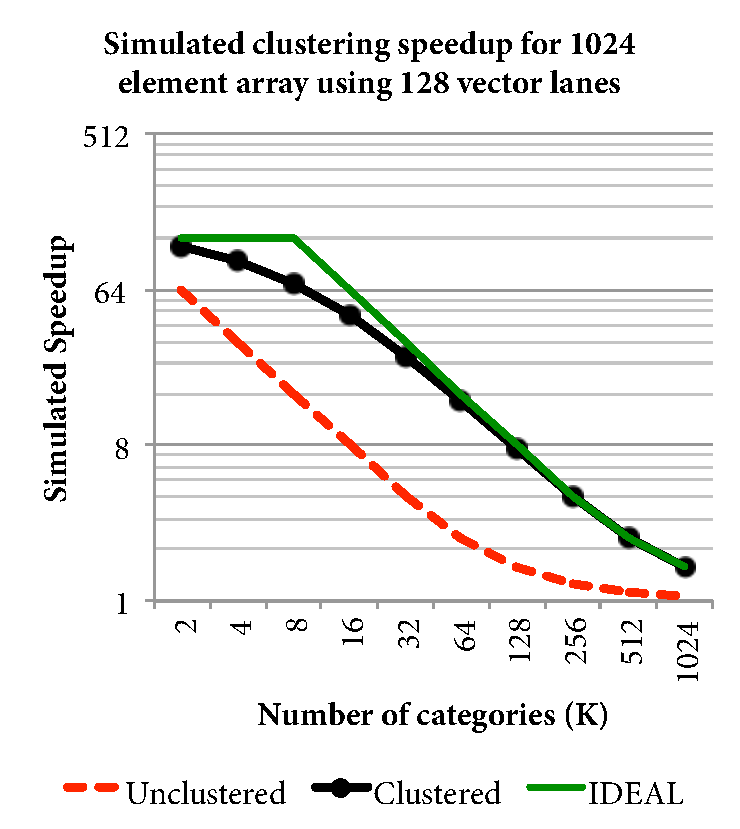
\includegraphics[trim=0 0 0 0,clip,width=0.32\columnwidth]{chapter6/simulatedclusteringspeedup/simulatedclusteringspeedup-7} }
\subfloat{  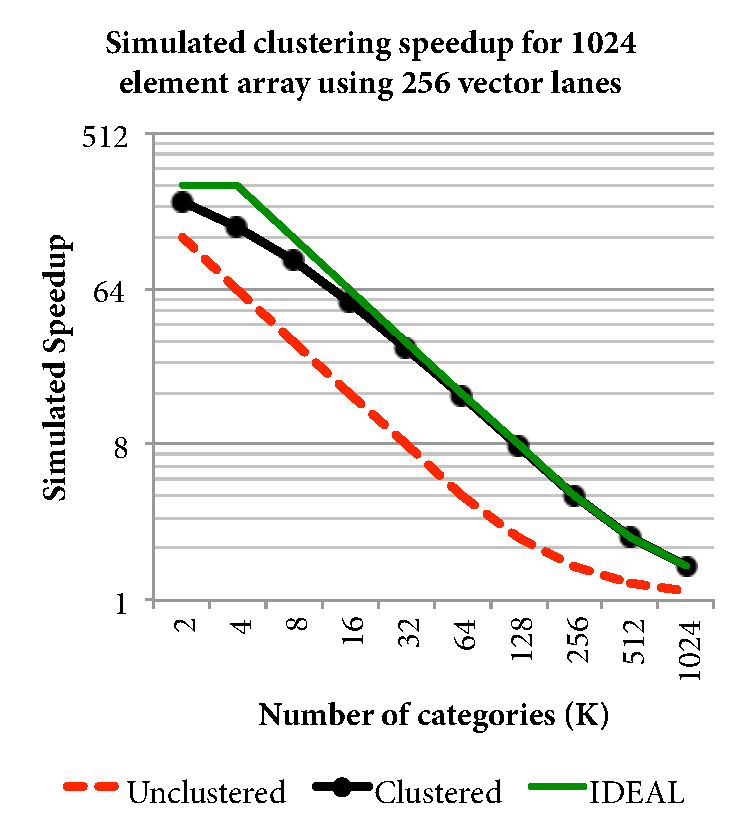
\includegraphics[trim=0 0 0 0,clip,width=0.32\columnwidth]{chapter6/simulatedclusteringspeedup/simulatedclusteringspeedup-8} }
\subfloat{  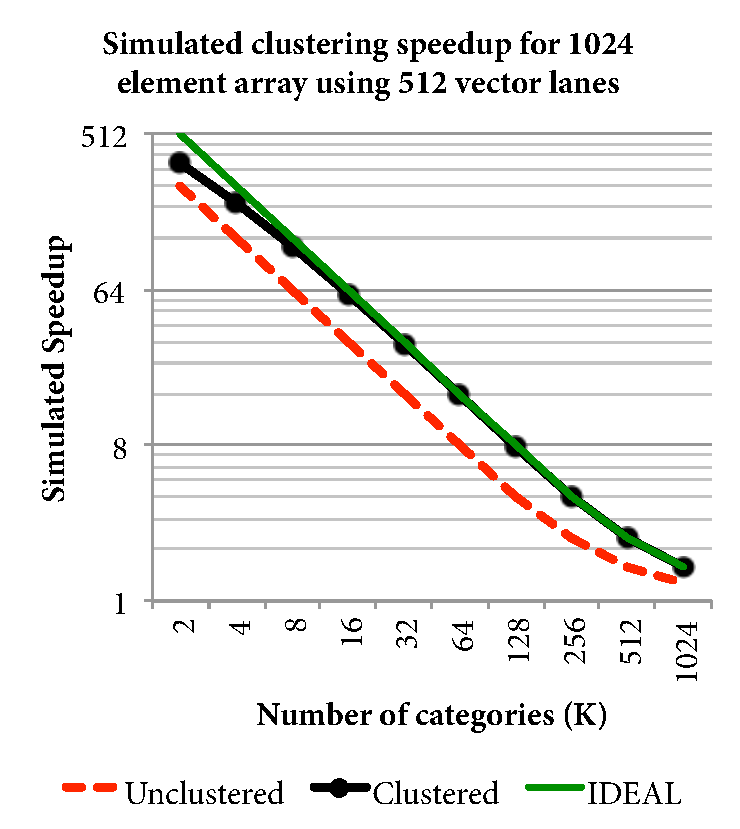
\includegraphics[trim=0 0 0 0,clip,width=0.32\columnwidth]{chapter6/simulatedclusteringspeedup/simulatedclusteringspeedup-9} } \\
\caption{\textbf{blah}}
\label{fig:simulatedclusteringspeedup}
\end{figure}





\subsection{The Problem}
The problem we address stems from layout being a computation where the instructions for each node are heavily input dependent. The intuition can be seen in contrasting the visual appearance of a webpage vs. a data visualization. Different parts of a webpage look quite different from one another, which suggests sensitivity to values in the input tree, while a visualization looks self-similar and thus does not use widely different instructions for different nodes.  For an example of divergence, an HBox's width is the sum of its children widths, while a VBox's is their maximum. The visit to a node (Figure~\ref{fig:compiled}) will diverge in instruction selection based on the node type.  

We ran a simulation to measure the performance cost of the divergence. Assuming a uniform distribution of types of nodes in a level, as the number of types of nodes go up ($K$), the probability that all of the nodes in a group share the same instructions drops exponentially. Figure~\ref{fig:simulatedclusteringspeedup} shows the simulated speedup for SIMD evaluation over a tree level of 1024 nodes on computer architectures with varying SIMD lengths. The x axis of each chart represents the number of types and the y axis is the speedup. As the number of choices increase, the benefit of the na\i{v}e breadth-first schedule (red line) decreases. It is far from the ideal speedup, which we estimated as a function of the SIMD length of the architecture (maximal parallel speedup, contributing the horizontal portion of the green lines) and the expected number of different categories (mandatory divergences, contributing the diagonal portion). 

\subsection{Code Clustering}
Our solution is to cluster nodes of a level based on the values of attributes that influence the flow of control. SIMD evaluation of the nodes in a cluster will be free of instruction divergence. Furthermore, by changing the data representation to match the clustered schedule, memory accesses will also be coalesced. We first focus on applying the clustering transformation to the code.



\newsavebox{\bfsClusteredVisitor}
\begin{lrbox}{\bfsClusteredVisitor}% Store first listing
\begin{lstlisting}[mathescape,language=C++,morekeywords={spawn,join,reverse,parallel_for}]
void parPreClustered(void (*visit)(Prod &), List<List<Array<Prod>>>  &levels) {
  for (List<Prod> level in levels)
  	for (Array<Prod> cluster in level)
  		parallel_for (Prod p in cluster)
			visit(p)
}
\end{lstlisting}
\end{lrbox}

\begin{figure}
 \usebox{\bfsClusteredVisitor}  
\caption{\textbf{ASDF.}}
\label{fig:clusteredeval}
\end{figure}


\newsavebox{\clusterUnswitchA}
\begin{lrbox}{\clusterUnswitchA}% Store first listing
\begin{lstlisting}[mathescape]
Prod firstProd = cluster[0]
parallel_for (prod in Cluster) {
  switch (firstProd.type) {
    case S $\rightarrow$ HBOX:  break;
    case HBOX $\rightarrow$ $\epsilon$:
      HBOX.w = input(); HBOX.h = input(); break;
    case HBOX $\rightarrow$ HBOX$_1$ HBOX$_2$:
      HBOX$_0$.w = HBOX$_1$.w + HBOX$_2$.w;
      HBOX$_0$.h = MAX(HBOX$_1$.h, HBOX$_2$.h);
      break;
  }
 }
\end{lstlisting}
\end{lrbox}

\newsavebox{\clusterUnswitchB}
\begin{lrbox}{\clusterUnswitchB}% Store first listing
\begin{lstlisting}[mathescape]
Prod firstProd = cluster[0]
  switch (firstProd.type) {
    case S $\rightarrow$ HBOX:  break;
    case HBOX $\rightarrow$ $\epsilon$:
      parallel_for (prod in Cluster) {
          HBOX.w = input(); HBOX.h = input();
     }
      break;
    case HBOX $\rightarrow$ HBOX$_1$ HBOX$_2$:
      parallel_for (prod in Cluster) {
        HBOX$_0$.w = HBOX$_1$.w + HBOX$_2$.w;
        HBOX$_0$.h = MAX(HBOX$_1$.h, HBOX$_2$.h);
      }
      break;
  }
 }
\end{lstlisting}
\end{lrbox}



\begin{figure}
\subfloat[\textbf{Clustered dispatch.}]{ \usebox{\clusterUnswitchA} } 
\subfloat[\textbf{Unswitched dispatch}.]{\usebox{\clusterUnswitchB} } 
\caption{\textbf{Loop transformations to exploit clustering for vectorization.}}
\label{fig:clusteringunswitching}
\end{figure}


Figure~\ref{fig:clusteredeval} shows the clustered evaluation variant of the MIMD $parPre$ traversal of Figure~\ref{fig:hboxall}. The traversal schedule is different because the order is based on the clustering rather than breadth-first index. Changing the order is safe because the original loop was parallel with no dependencies between elements.  Computing over clusters guarantees that all calls to a visit dispatch function in the parallel inner loop (e.g., of $visit1$) will branch to the same switch statement case. This modified schedule avoids instruction divergence. 

Our loop transformation can be understood as a use of loop unswitching, which is a common transformation for improving parallelization. Loop unswitching lifts a conditional out of a loop by duplicating the  loop inside of both cases of the conditional. Clustering establishes the invariant of being able to inspect the first item of a collection sufficing for performing unswitching for a loop over all of the items. Figure~\ref{fig:clusteringunswitching} separates our transformation of $visit1$ (Figure \ref{fig:hboxall}) into using the same exemplar for the dispatch and then loop unswitching.

Clustering is with respect to input attributes that influence control flow, which may be more than the node type. For example, in our parallelization of the C3 layout engine, we found that the engine author combined the logic of multiple box types into one visit function because the variants shared a lot of code. He instead used multiple node flags to guide instruction selection. Both the node type and various other node attributes influenced control flow, and therefore our clustering condition was on whether they were all equal. Using all of the attributes led to too granular of a clustering condition, so we manually tuned the choice of attributes.

\subsection{Data Clustering}
The data representation should be modified to match the clustering order. The benefit is coalesced memory accesses, but overhead costs in performing the clustering should be considered.

Our algorithm matches the data representation order to the schedule by placing nodes of a cluster into the same contiguous array. Parallel reads and are coalesced, such as the inspection of the node type for the visit dispatch. Parallel writes are likewise coalesced.

Reordering data is expensive as all of the data is moved. In the case of our data visualization system, we can avoid the cost because the data is preprocessed on our server. For webpage layout, the client performs clustering, which we optimize enough such that the cost is outweighed by the subsequent performance improvements.

We optimize reordering with a simple parallel two-pass technique. The first pass traverses each level in parallel to compute the cluster for each node and tabulate the cluster sizes for each tree level. The second pass again traverses each level in parallel, and as each node is traversed, copies it into the next free slot of the appropriate cluster. Even finer-grained parallelization is possible, but this algorithm was sufficient for lowering reordering costs enough to be amortized.

\subsection{Nested Clustering}
Clustering can also be used to address divergences induced by computations over neighboring nodes. They avoidable irregularities can take several forms:

\begin{itemize}
\item \textbf{Branches.} For the case of webpage layout, we saw cases where attributes of the parent node or children node influence instruction selection, such as whether to include a child node in a width computation. The properties can be included in the clustering condition to eliminate the corresponding instruction divergences. 

\item \textbf{Load imbalance in loops.} One node may have no children while another may have many. If the layout computation involves a loop, SIMD evaluation will perform the two loops in lock-step. Thus, as the nodes have different amounts of children, the SIMD lanes devoted to the first child will not be utilized: this is a load balancing problem. The number of children can be included in the clustering condition to eliminate load imbalance.

\item \textbf{Random memory access in loops.} A further issue with lock-step loops over child nodes is memory divergence. A breadth-first layout would provide strided memory access, but if each level is clustered, the locations of a node's children may be random without further aid. We found a \emph{nested} solution where \emph{subtrees} are assigned to clusters. Instead of just associating nodes of a level with a cluster, our algorithm then treats the nodes of a cluster as roots. It recursively expands a subtree such that all of the cluster nodes share it (with respect to the attributes influencing control flow). The data layout follows the nested clustering, so parallel memory accesses to the children of nodes will be coalesced. 
\end{itemize}

Each of these clusterings introduce an invariant for a cluster for optimizing performance within that cluster. However, the clustering condition is more discriminating.  Cluster sizes may decrease, which would  significantly decrease  performance if cluster size shrinks below vector length size. Our evaluation explores these options in practice.
